\documentclass[tikz,border=14pt]{standalone}
\usepackage[utf8]{inputenc}
\usepackage[T1]{fontenc}
\usepackage[scaled=.95]{helvet}
\usepackage{amsmath}
\renewcommand{\familydefault}{\sfdefault}
\usetikzlibrary{arrows.meta,positioning,calc,shapes.geometric,fit,backgrounds,decorations.pathreplacing}
\definecolor{bg}{HTML}{05070A}
\definecolor{panel}{HTML}{0B1220}
\definecolor{node}{HTML}{0F1A24}
\definecolor{teal}{HTML}{14B8A6}
\definecolor{tealD}{HTML}{0E756D}
\definecolor{brandred}{HTML}{DD0000}
\definecolor{silver}{HTML}{C9D6DE}
\definecolor{mute}{HTML}{8A97A6}
\ifx\LANG\undefined\def\LANG{p}\fi
\def\T#1#2{\if\LANG p#1\else#2\fi}
\newcommand{\subx}[1]{{\color{mute}\scriptsize #1}}
\tikzset{
  every node/.style={text=silver,font=\sffamily},
  blk/.style={draw=tealD,fill=node,rounded corners=7pt,line width=1pt,align=center,inner sep=7pt,minimum width=3.3cm,minimum height=1.9cm,font=\sffamily\small},
  hot/.style={blk,draw=brandred},
  ttl/.style={text=white,font=\sffamily\bfseries\large},
  num/.style={circle,fill=teal,text=bg,font=\sffamily\bfseries\footnotesize,inner sep=2pt,minimum size=15pt},
  sub/.style={text=mute,font=\sffamily\scriptsize},
  arr/.style={-{Stealth[length=7pt]},teal,line width=1.4pt},
}
\newcommand{\panel}[1]{\begin{scope}[on background layer]\node[fit=#1,inner sep=16pt,fill=bg,rounded corners=12pt]{};\end{scope}}

\begin{document}
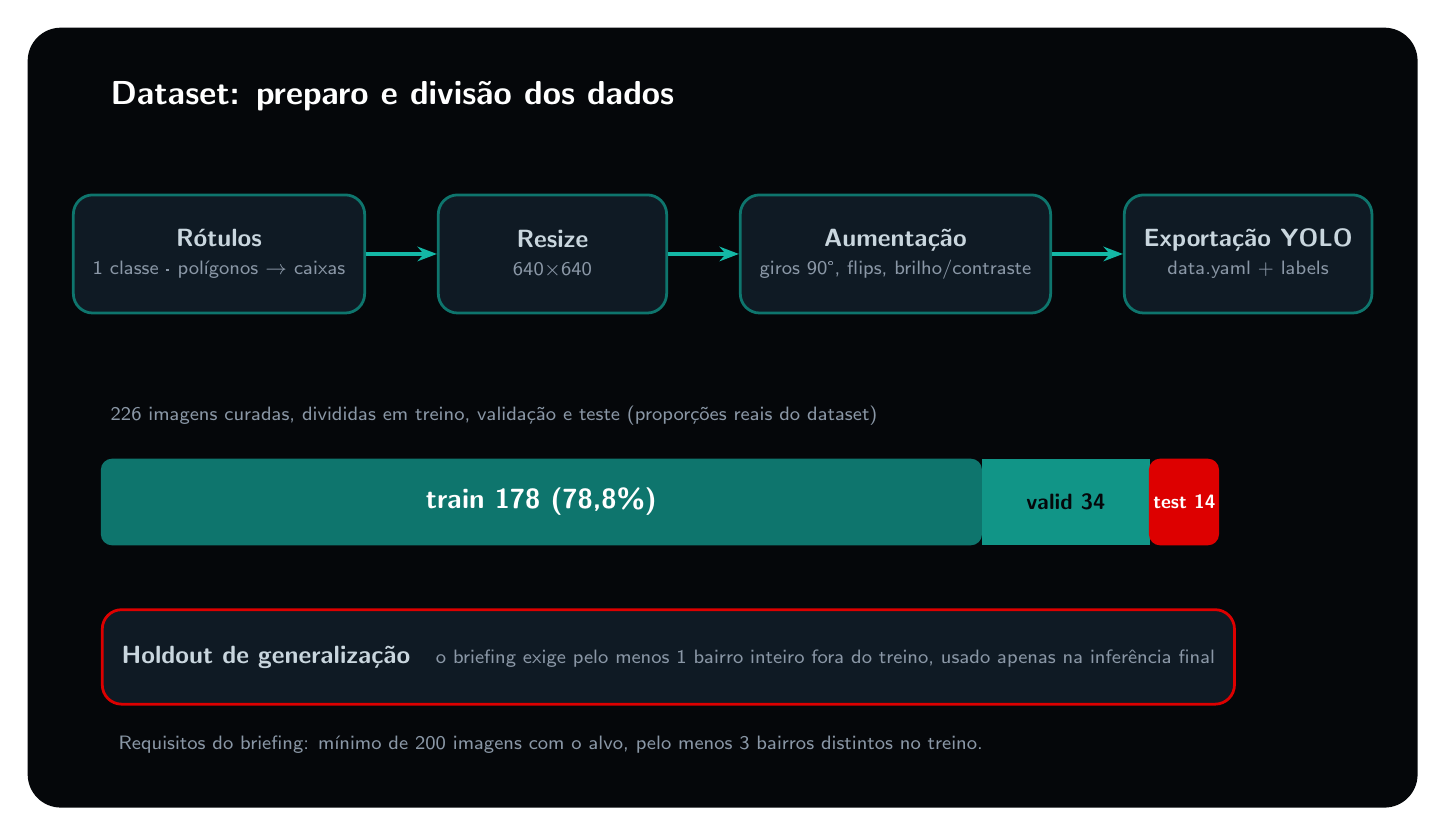
\begin{tikzpicture}
\node[ttl,anchor=west] (t) at (0,3.2) {\T{Dataset: preparo e divisão dos dados}{Dataset: preparation and data split}};
% preprocessing chain
\node[blk,minimum width=2.9cm,minimum height=1.5cm] (a) at (1.5,1.2) {\textbf{\T{Rótulos}{Labels}}\\[-1pt]\subx{\T{1 classe · polígonos $\rightarrow$ caixas}{1 class · polygons $\rightarrow$ boxes}}};
\node[blk,minimum width=2.9cm,minimum height=1.5cm,right=0.9cm of a] (b) {\textbf{Resize}\\[-1pt]\subx{640$\times$640}};
\node[blk,minimum width=2.9cm,minimum height=1.5cm,right=0.9cm of b] (c) {\textbf{\T{Aumentação}{Augmentation}}\\[-1pt]\subx{\T{giros 90°, flips, brilho/contraste}{90° rotations, flips, brightness/contrast}}};
\node[blk,minimum width=2.9cm,minimum height=1.5cm,right=0.9cm of c] (d) {\textbf{\T{Exportação YOLO}{YOLO export}}\\[-1pt]\subx{data.yaml + labels}};
\foreach \x/\y in {a/b,b/c,c/d} \draw[arr] (\x) -- (\y);
% split bar
\def\W{14.2}
\fill[tealD,rounded corners=4pt] (0,-1.4) rectangle (0.788*\W,-2.5);
\fill[teal!80!bg] (0.788*\W,-1.4) rectangle (0.938*\W,-2.5);
\fill[brandred,rounded corners=4pt] (0.938*\W-0.01,-1.4) rectangle (\W,-2.5);
\node[text=white,font=\sffamily\bfseries] at (0.394*\W,-1.95) {train 178 (\T{78{,}8}{78.8}\%)};
\node[text=bg,font=\sffamily\bfseries\footnotesize] at (0.863*\W,-1.95) {valid 34};
\node[text=white,font=\sffamily\bfseries\scriptsize] at (0.969*\W,-1.95) {test 14};
\node[sub,anchor=west] at (0,-0.85) {\T{226 imagens curadas, divididas em treino, validação e teste (proporções reais do dataset)}{226 curated images split into train, validation and test (actual dataset proportions)}};
% holdout
\node[blk,hot,minimum width=\W cm,minimum height=1.2cm,align=left,anchor=north west] (h) at (0,-3.3) {\textbf{\T{Holdout de generalização}{Generalization holdout}}\quad \subx{\T{o briefing exige pelo menos 1 bairro inteiro fora do treino, usado apenas na inferência final}{the briefing requires at least 1 whole neighborhood excluded from training, used only for final inference}}};
\node[sub,anchor=west] (n) at ($(h.south west)+(0.1,-0.5)$) {\T{Requisitos do briefing: mínimo de 200 imagens com o alvo, pelo menos 3 bairros distintos no treino.}{Briefing requirements: at least 200 images containing the target, at least 3 distinct neighborhoods in training.}};
\panel{(t)(a)(b)(c)(d)(h)(n)}
\end{tikzpicture}
\end{document}
